% Chapter 3

\chapter{METHODOLOGICAL FRAMEWORKS} % Main chapter title

\label{Chapter3} % Change X to a consecutive number; for referencing this chapter elsewhere, use \ref{ChapterX}

\lhead{Chapter 3. \emph{Methodological Frameworks}} % Change X to a consecutive number; this is for the header on each page - perhaps a shortened title

%----------------------------------------------------------------------------------------
%	SECTION 1
%----------------------------------------------------------------------------------------



%\begin{figure}[htbp]
%	\centering
%	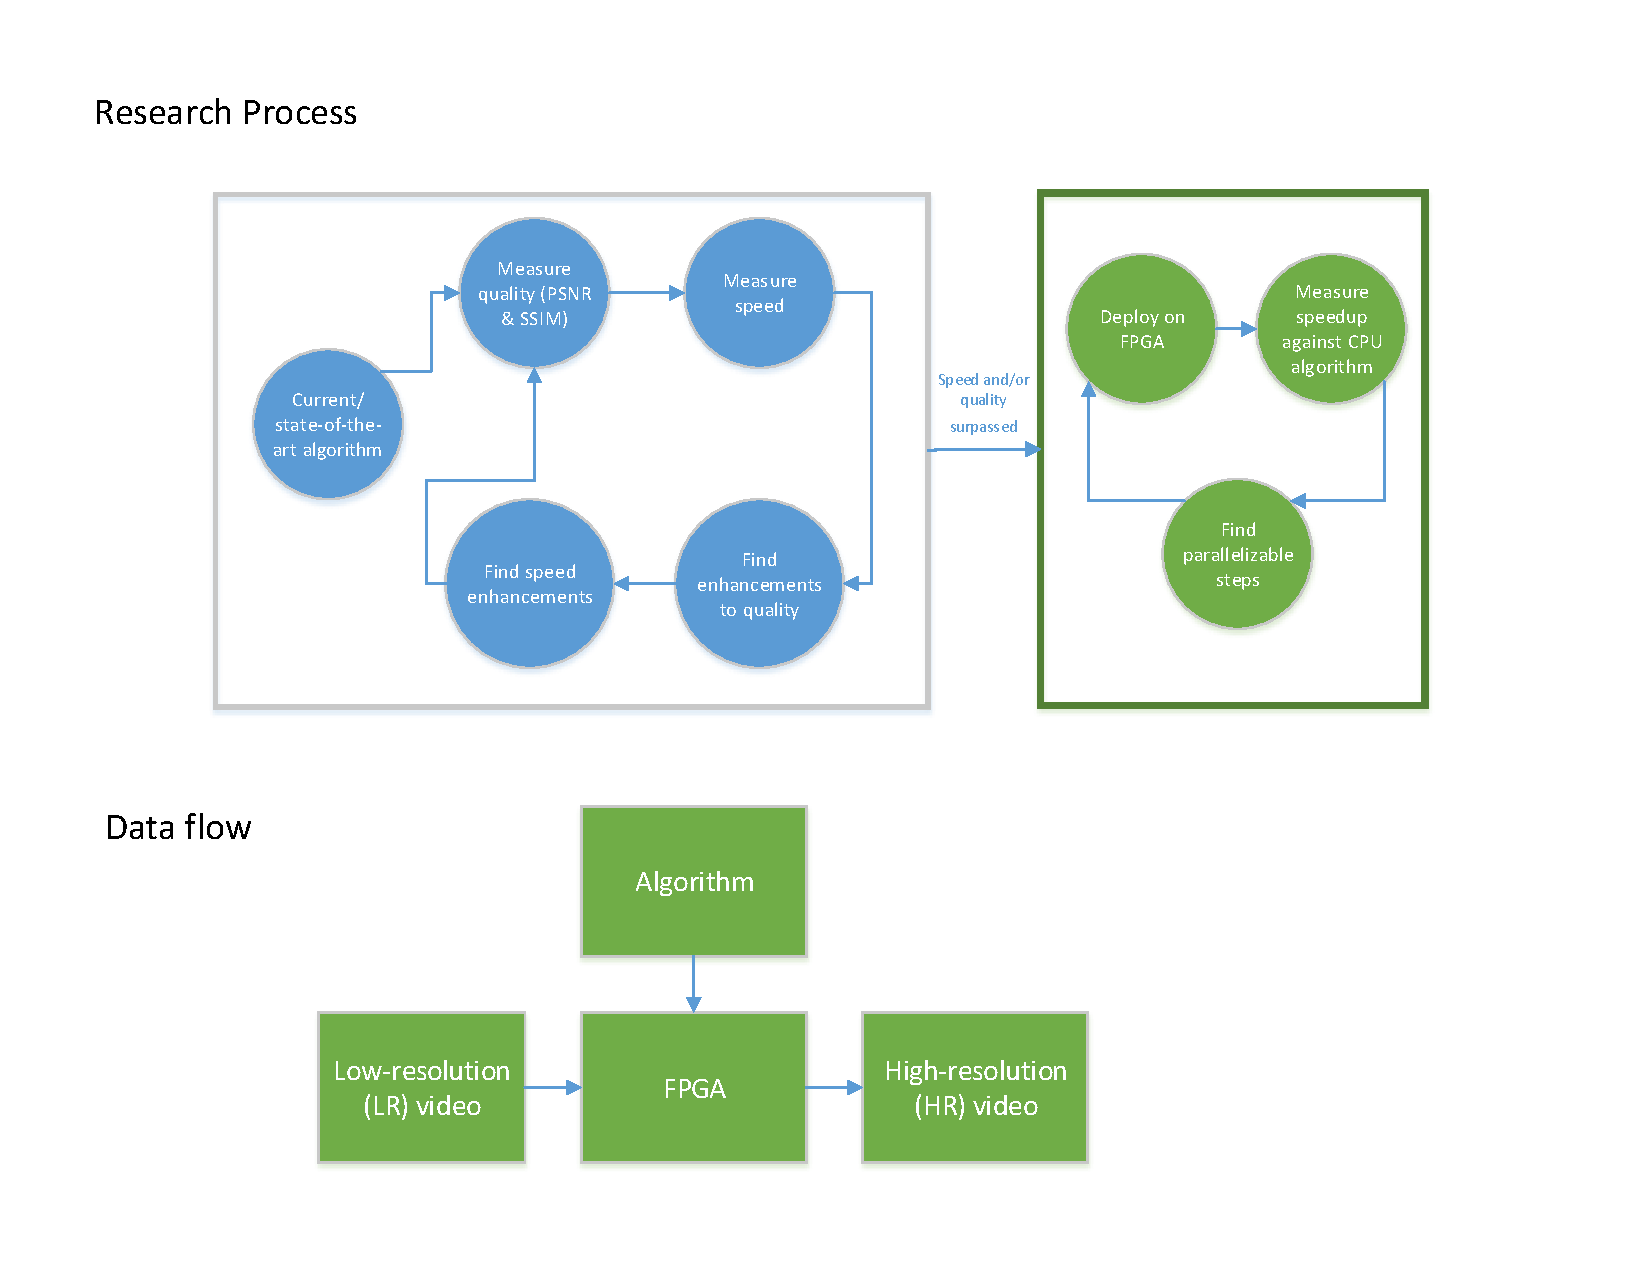
\includegraphics{Figures/framework.pdf}
%	\rule{35em}{0.2pt}
%	\caption[Conceptual Framework]{Conceptual Framework of the Study.}
%	\label{fig:Framework}
%\end{figure}



%-----------------------------------
%	SUBSECTION 1
%-----------------------------------
\section{Theoretical Considerations}
Given a reference image \textit{a} and a test image \textit{b}, both of the same size \textit{M}x\textit{N},the PSNR is computed using the following equation \citep{Hore2010}:

\begin{equation}
PSNR(a,b) = 20 \log_{10}\frac{255}{\sqrt{MSE(a,b)}}
\end{equation}

where
\begin{equation}
MSE(a,b) = \frac{1}{MN} \sum\limits_{i=1}^{M} \sum\limits_{j=1}^{N} (a_{ij}-b_{ij})^2
\end{equation}

The SSIM is computed using the following equation \citep{Hore2010}:

\begin{equation}
SSIM(a,b) = l(a,b) c(a,b) s(a,b)
\end{equation}

where
\begin{eqnarray}
l(a,b) = \frac{2\mu_a\mu_b+C_1}{\mu_a^2+\mu_b^2+C_1} \label{eqn:luminance_ssim}\\
c(a,b) = \frac{2\sigma_a\sigma_b+C_2}{\sigma_a^2+\sigma_b^2+C_2}\label{eqn:contrast_ssim}\\
s(a,b) = \frac{\sigma_{ab}+C_3}{\sigma_a\sigma_b+C_3}\label{eqn:structure_ssim}
\end{eqnarray}

Equation \ref{eqn:luminance_ssim} measures the similarity in luminance and is equal to 1 only if $\mu_a=\mu_b$.
Similarly, equation \ref{eqn:contrast_ssim} compares the standard deviation of the two images (which corresponds to the contrast). 
It will only equal to 1 if $\sigma_a=\sigma_b$.
The structure comparison equation (\ref{eqn:structure_ssim}) measures the correlation between the images using the covariance $\sigma_{ab}$ between them.

The FSIM is computed using the following equation \citep{Zhang2011a}:

\begin{equation}
\frac{\sum_{x\in\Omega}S_L(\mathbf{x})\cdot PC_m(\mathbf{x})}{{\sum_{x\in\Omega}PC_m(\mathbf{x})}}
\end{equation}

where $\Omega$ is the whole spatial image domain.
$S_L(\mathbf{x})$

\section{Algorithm Framework}

% Explain the framework
Figure \ref{fig:algoframe} summarizes the flow of the proposed algorithm.
The major components of this algorithm are the deblurring module, the temporal consistency module, and the edge-preservation module.
The deblurring module removes image blur caused by motion and the camera sensor.
The temporal consistency module ensures that successive video frames are consistently super-resolved with respect to time.
It uses the preceding HR frame to accomplish this task.
The edge-preservation module takes the finer details of the LR video frames and interpolates the HR version of the edges.
A final reconstruction step incorporates output all the three major modules to generate the HR frame sequence.

% Place figure here
\begin{figure}[!ht]
	\centering
	\includegraphics[scale=0.7]{Figures/ALGO_FRAMEWORK.png}
	\caption[]{Framework for the Algorithm.}
	\label{fig:algoframe}
\end{figure}


%-----------------------------------
%	SUBSECTION 2
%-----------------------------------


\section{Hardware Framework}
Figure \ref{fig:hardframe} illustrates the flow of data across the hardware devices to be used in the study.
A video source such as a camera or prerecorded file will be sent for super-resolution on the SoC, which will then display the result on the monitor in real-time.
Initially a conventional computer will serve as the development and evaluation  environment for the SR algorithm.
A revised version of the algorithm can then be sent to the SoC for further testing and fine-tuning.

\begin{figure}[!ht]
	\centering
	\includegraphics[scale=0.7]{Figures/HARDWARE_FRAMEWORK.png}
	\caption[]{Framework for Hardware Implementation.}
	\label{fig:hardframe}
\end{figure}

% Explain the framework



%----------------------------------------------------------------------------------------
%	SECTION 2
%----------------------------------------------------------------------------------------
